% Options for packages loaded elsewhere
\PassOptionsToPackage{unicode}{hyperref}
\PassOptionsToPackage{hyphens}{url}
%
\documentclass[
]{book}
\usepackage{amsmath,amssymb}
\usepackage{lmodern}
\usepackage{ifxetex,ifluatex}
\ifnum 0\ifxetex 1\fi\ifluatex 1\fi=0 % if pdftex
  \usepackage[T1]{fontenc}
  \usepackage[utf8]{inputenc}
  \usepackage{textcomp} % provide euro and other symbols
\else % if luatex or xetex
  \usepackage{unicode-math}
  \defaultfontfeatures{Scale=MatchLowercase}
  \defaultfontfeatures[\rmfamily]{Ligatures=TeX,Scale=1}
\fi
% Use upquote if available, for straight quotes in verbatim environments
\IfFileExists{upquote.sty}{\usepackage{upquote}}{}
\IfFileExists{microtype.sty}{% use microtype if available
  \usepackage[]{microtype}
  \UseMicrotypeSet[protrusion]{basicmath} % disable protrusion for tt fonts
}{}
\makeatletter
\@ifundefined{KOMAClassName}{% if non-KOMA class
  \IfFileExists{parskip.sty}{%
    \usepackage{parskip}
  }{% else
    \setlength{\parindent}{0pt}
    \setlength{\parskip}{6pt plus 2pt minus 1pt}}
}{% if KOMA class
  \KOMAoptions{parskip=half}}
\makeatother
\usepackage{xcolor}
\IfFileExists{xurl.sty}{\usepackage{xurl}}{} % add URL line breaks if available
\IfFileExists{bookmark.sty}{\usepackage{bookmark}}{\usepackage{hyperref}}
\hypersetup{
  pdftitle={Cours Physique-Chimie (Spécialité)},
  pdfauthor={Cyril DENIS},
  hidelinks,
  pdfcreator={LaTeX via pandoc}}
\urlstyle{same} % disable monospaced font for URLs
\usepackage[left=2cm,right=2cm,top=2cm,bottom=2cm]{geometry}
\usepackage{color}
\usepackage{fancyvrb}
\newcommand{\VerbBar}{|}
\newcommand{\VERB}{\Verb[commandchars=\\\{\}]}
\DefineVerbatimEnvironment{Highlighting}{Verbatim}{commandchars=\\\{\}}
% Add ',fontsize=\small' for more characters per line
\usepackage{framed}
\definecolor{shadecolor}{RGB}{248,248,248}
\newenvironment{Shaded}{\begin{snugshade}}{\end{snugshade}}
\newcommand{\AlertTok}[1]{\textcolor[rgb]{0.94,0.16,0.16}{#1}}
\newcommand{\AnnotationTok}[1]{\textcolor[rgb]{0.56,0.35,0.01}{\textbf{\textit{#1}}}}
\newcommand{\AttributeTok}[1]{\textcolor[rgb]{0.77,0.63,0.00}{#1}}
\newcommand{\BaseNTok}[1]{\textcolor[rgb]{0.00,0.00,0.81}{#1}}
\newcommand{\BuiltInTok}[1]{#1}
\newcommand{\CharTok}[1]{\textcolor[rgb]{0.31,0.60,0.02}{#1}}
\newcommand{\CommentTok}[1]{\textcolor[rgb]{0.56,0.35,0.01}{\textit{#1}}}
\newcommand{\CommentVarTok}[1]{\textcolor[rgb]{0.56,0.35,0.01}{\textbf{\textit{#1}}}}
\newcommand{\ConstantTok}[1]{\textcolor[rgb]{0.00,0.00,0.00}{#1}}
\newcommand{\ControlFlowTok}[1]{\textcolor[rgb]{0.13,0.29,0.53}{\textbf{#1}}}
\newcommand{\DataTypeTok}[1]{\textcolor[rgb]{0.13,0.29,0.53}{#1}}
\newcommand{\DecValTok}[1]{\textcolor[rgb]{0.00,0.00,0.81}{#1}}
\newcommand{\DocumentationTok}[1]{\textcolor[rgb]{0.56,0.35,0.01}{\textbf{\textit{#1}}}}
\newcommand{\ErrorTok}[1]{\textcolor[rgb]{0.64,0.00,0.00}{\textbf{#1}}}
\newcommand{\ExtensionTok}[1]{#1}
\newcommand{\FloatTok}[1]{\textcolor[rgb]{0.00,0.00,0.81}{#1}}
\newcommand{\FunctionTok}[1]{\textcolor[rgb]{0.00,0.00,0.00}{#1}}
\newcommand{\ImportTok}[1]{#1}
\newcommand{\InformationTok}[1]{\textcolor[rgb]{0.56,0.35,0.01}{\textbf{\textit{#1}}}}
\newcommand{\KeywordTok}[1]{\textcolor[rgb]{0.13,0.29,0.53}{\textbf{#1}}}
\newcommand{\NormalTok}[1]{#1}
\newcommand{\OperatorTok}[1]{\textcolor[rgb]{0.81,0.36,0.00}{\textbf{#1}}}
\newcommand{\OtherTok}[1]{\textcolor[rgb]{0.56,0.35,0.01}{#1}}
\newcommand{\PreprocessorTok}[1]{\textcolor[rgb]{0.56,0.35,0.01}{\textit{#1}}}
\newcommand{\RegionMarkerTok}[1]{#1}
\newcommand{\SpecialCharTok}[1]{\textcolor[rgb]{0.00,0.00,0.00}{#1}}
\newcommand{\SpecialStringTok}[1]{\textcolor[rgb]{0.31,0.60,0.02}{#1}}
\newcommand{\StringTok}[1]{\textcolor[rgb]{0.31,0.60,0.02}{#1}}
\newcommand{\VariableTok}[1]{\textcolor[rgb]{0.00,0.00,0.00}{#1}}
\newcommand{\VerbatimStringTok}[1]{\textcolor[rgb]{0.31,0.60,0.02}{#1}}
\newcommand{\WarningTok}[1]{\textcolor[rgb]{0.56,0.35,0.01}{\textbf{\textit{#1}}}}
\usepackage{longtable,booktabs,array}
\usepackage{calc} % for calculating minipage widths
% Correct order of tables after \paragraph or \subparagraph
\usepackage{etoolbox}
\makeatletter
\patchcmd\longtable{\par}{\if@noskipsec\mbox{}\fi\par}{}{}
\makeatother
% Allow footnotes in longtable head/foot
\IfFileExists{footnotehyper.sty}{\usepackage{footnotehyper}}{\usepackage{footnote}}
\makesavenoteenv{longtable}
\usepackage{graphicx}
\makeatletter
\def\maxwidth{\ifdim\Gin@nat@width>\linewidth\linewidth\else\Gin@nat@width\fi}
\def\maxheight{\ifdim\Gin@nat@height>\textheight\textheight\else\Gin@nat@height\fi}
\makeatother
% Scale images if necessary, so that they will not overflow the page
% margins by default, and it is still possible to overwrite the defaults
% using explicit options in \includegraphics[width, height, ...]{}
\setkeys{Gin}{width=\maxwidth,height=\maxheight,keepaspectratio}
% Set default figure placement to htbp
\makeatletter
\def\fps@figure{htbp}
\makeatother
\setlength{\emergencystretch}{3em} % prevent overfull lines
\providecommand{\tightlist}{%
  \setlength{\itemsep}{0pt}\setlength{\parskip}{0pt}}
\setcounter{secnumdepth}{5}
\usepackage{booktabs}
\usepackage{siunitx}
\usepackage{chemfig}
%\usepackage{amssymb,amsmath}
\usepackage[french]{babel}
\usepackage{eurosym}
\newtheorem{definition}{Définition}
\newtheorem{theorem}{Application}



\renewcommand\thesection       {\Roman{section}.}
\renewcommand\thesubsection    {\thesection \arabic{subsection}.}
\renewcommand\thesubsubsection {\thesubsection \alph{subsubsection})}
\renewcommand\theparagraph     {\thesubsubsection.\arabic{paragraph}}
\renewcommand\thesubparagraph  {\theparagraph.\arabic{subparagraph}}
\setcounter{secnumdepth}{4}
\def\tightlist{}
\newcommand{\fiche}[3]{
	\begin{center}
		\textsc{#1}\\
		#2\hfill\textit{#3}
	\end{center}
	\hrule\vspace{\baselineskip}
}

\newcounter{numeroexo}
\newcommand{\exo}{\par\noindent\stepcounter{numeroexo}
	\hspace{-.25cm}\fbox{\textbf{Exercice \arabic{numeroexo}}}\quad}
% Code pour boite noire
\usepackage{tcolorbox}

\newtcolorbox{blackbox}{
  colback=red!10!white,
  colframe=gray,
  coltext=black,
  boxsep=5pt,
  arc=4pt}
\ifluatex
  \usepackage{selnolig}  % disable illegal ligatures
\fi
\usepackage[]{natbib}
\bibliographystyle{apalike}

\title{Cours Physique-Chimie (Spécialité)}
\author{Cyril DENIS}
\date{2021-07-04}

\begin{document}
\maketitle

{
\setcounter{tocdepth}{1}
\tableofcontents
}
\hypertarget{prerequisites}{%
\chapter{Prerequisites}\label{prerequisites}}

This is a \emph{sample} book written in \textbf{Markdown}. You can use anything that Pandoc's Markdown supports, e.g., a math equation \(a^2 + b^2 = c^2\).

$4\times 3$
\\

\begin{figure}
\centering

\includegraphics{~/Desktop/termniale/figures/tasse-a-mesurer.png}
\caption{Légende}
\end{figure}

\[E = mc^2\]

The \textbf{bookdown} package can be installed from CRAN or Github:

\exo

\hypertarget{sous-section}{%
\section{sous section}\label{sous-section}}

\hypertarget{sou-sous-sedctpo}{%
\subsection{sou sous sedctpo,}\label{sou-sous-sedctpo}}

emzfe
\begin{theorem}
\protect\hypertarget{thm:unnamed-chunk-1}{}{\label{thm:unnamed-chunk-1} }Here is my theorem.
\end{theorem}

La mole est une unité de quantité de matière. C'est un nombre de choses.
Dans une mole il y a \(N_a\) (Nombre d'Avogadro) choses avec \(N_a=\SI{6,02e23}{\per\mole}\)\textbackslash{}
\textit{Analogie : Dans une douzaine d'oeufs, il y a douze oeufs.\\
Dans une mole d'oeufs, il y a $\SI{6,02e23}{}$ oeufs et dans une mole d'ions cuivre II, il y a $\SI{6,02e23}{}$  ions cuivre II.}\textbackslash{}

\begin{definition}
\protect\hypertarget{def:unnamed-chunk-2}{}{\label{def:unnamed-chunk-2} }Un court circuit est un circuit court..
\end{definition}

\begin{Shaded}
\begin{Highlighting}[]
\FunctionTok{install.packages}\NormalTok{(}\StringTok{"bookdown"}\NormalTok{)}
\CommentTok{\# or the development version}
\CommentTok{\# devtools::install\_github("rstudio/bookdown")}
\end{Highlighting}
\end{Shaded}

Remember each Rmd file contains one and only one chapter, and a chapter is defined by the first-level heading \texttt{\#}.

To compile this example to PDF, you need XeLaTeX. You are recommended to install TinyTeX (which includes XeLaTeX): \url{https://yihui.org/tinytex/}.

\begin{Shaded}
\begin{Highlighting}[]
\ImportTok{import}\NormalTok{ numpy }\ImportTok{as}\NormalTok{ np}
\ImportTok{import}\NormalTok{ matplotlib.pyplot }\ImportTok{as}\NormalTok{ plt}
\ImportTok{import}\NormalTok{ numpy.random }\ImportTok{as}\NormalTok{ rng}
\ImportTok{import}\NormalTok{ matplotlib.cm }\ImportTok{as}\NormalTok{ cm}
\ImportTok{from}\NormalTok{ matplotlib.animation }\ImportTok{import}\NormalTok{ FuncAnimation}

\NormalTok{radii}\OperatorTok{=}\NormalTok{(rng.random(}\BuiltInTok{int}\NormalTok{(}\FloatTok{1e3}\NormalTok{))}\OperatorTok{+}\DecValTok{1}\NormalTok{)}\OperatorTok{**}\DecValTok{2}
\NormalTok{iota}\OperatorTok{=}\DecValTok{2}\OperatorTok{*}\NormalTok{np.pi}\OperatorTok{*}\NormalTok{rng.random(}\BuiltInTok{int}\NormalTok{(}\FloatTok{1e3}\NormalTok{))}
\NormalTok{x\_posit}\OperatorTok{=}\NormalTok{np.sqrt(radii)}\OperatorTok{*}\NormalTok{np.cos(iota)}
\NormalTok{y\_posit}\OperatorTok{=}\NormalTok{np.sqrt(radii)}\OperatorTok{*}\NormalTok{np.sin(iota)}
\NormalTok{plt.plot(x\_posit, y\_posit, }\StringTok{\textquotesingle{}go\textquotesingle{}}\NormalTok{)}
\end{Highlighting}
\end{Shaded}

\begin{verbatim}
## [<matplotlib.lines.Line2D object at 0x7f9cb5c52c18>]
\end{verbatim}

\begin{Shaded}
\begin{Highlighting}[]
\NormalTok{plt.show()}
\end{Highlighting}
\end{Shaded}

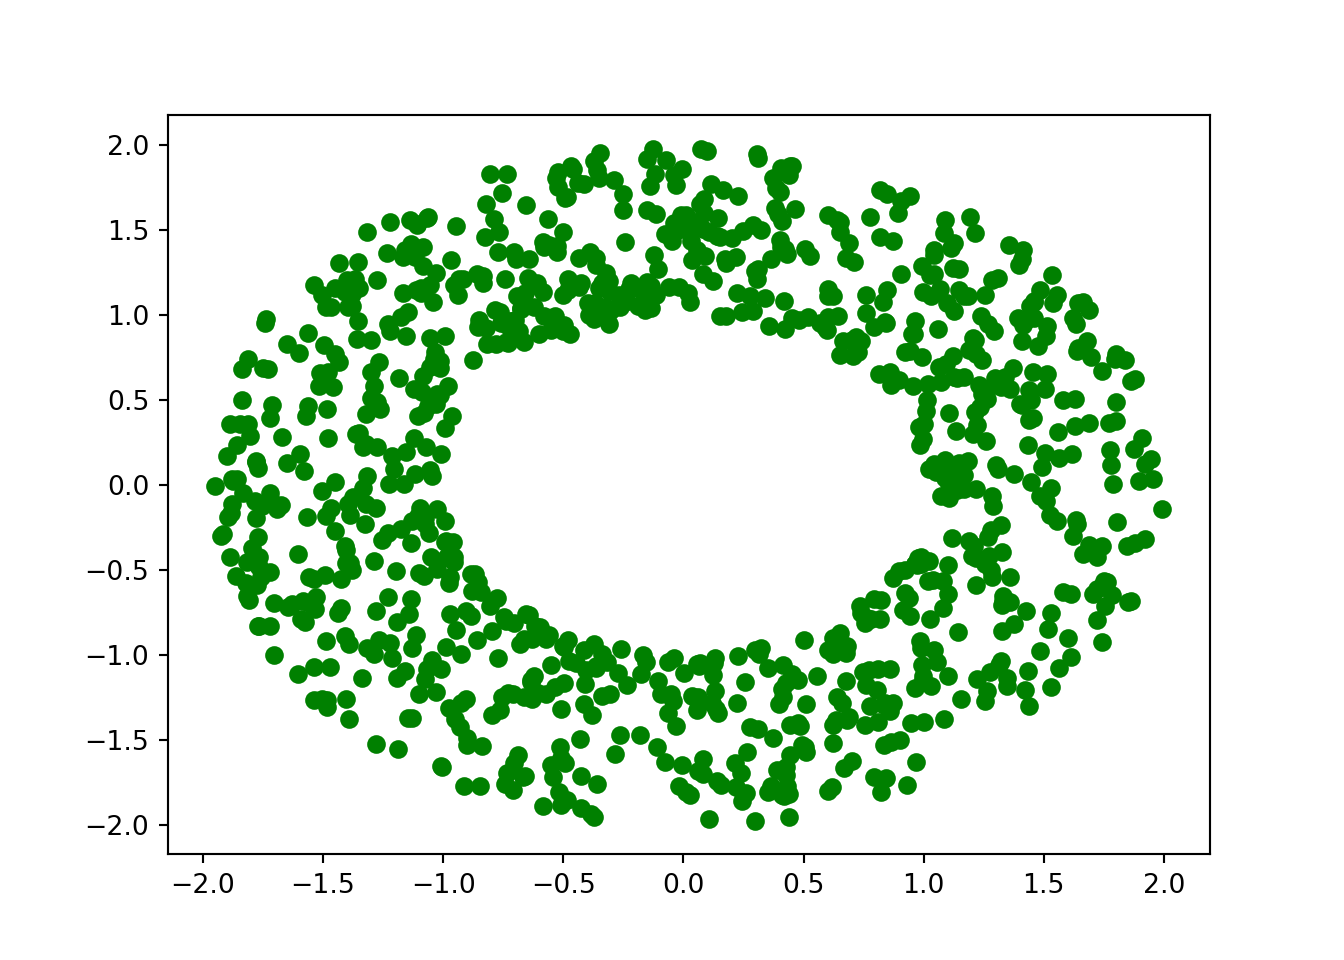
\includegraphics{book_files/figure-latex/unnamed-chunk-4-1.pdf}

\hypertarget{rappels-de-chimie}{%
\chapter*{Rappels de Chimie}\label{rappels-de-chimie}}
\addcontentsline{toc}{chapter}{Rappels de Chimie}

\hypertarget{calcul-de-quantituxe9-de-matiuxe8re}{%
\section{Calcul de quantité de matière}\label{calcul-de-quantituxe9-de-matiuxe8re}}

\hypertarget{quantituxe9-de-matiuxe8re-et-nombre-de-particules}{%
\subsection{Quantité de matière et Nombre de particules}\label{quantituxe9-de-matiuxe8re-et-nombre-de-particules}}

\begin{enumerate}
\def\labelenumi{\arabic{enumi}.}
\tightlist
\item
  Faire un schéma représentant une mole d'atome de carbone.
\item
  Un échantillon de fer contient \(12.10^{22}\) atomes de fer. Quelle est la quantité de matière contenue dans cette échantillon.
\item
  Combien de molécules contient un échantillon de 0,10 mol d'eau.
\end{enumerate}

\hypertarget{masse-et-masse-molaire}{%
\subsection{Masse et Masse Molaire}\label{masse-et-masse-molaire}}

\begin{enumerate}
\def\labelenumi{\arabic{enumi}.}
\tightlist
\item
  Calculer la masse molaire des espèces chimique suivantes: \(H_2O\), \(CO_2\), \(C_6H_{12}O_6\), \(NO_3^{-}\) et \(Cu(OH)_2\).
\item
  On considère un échantillon de glucose \(C_6H_{12}O_6\) de masse \(m=20\) g. Quelle est la quantité de matière contenue dans cet échantillon ?
\item
  Déterminer la masse de l'échantillon de fer contenant la même quantité de matière que l'échantillon précédent de glucose. On donne \(M_{Fe}=56\) g/mol.
\item
  Expliquer simplement pourquoi deux échantillons contenant la même quantité de matière n'ont pas en général la même masse.
\end{enumerate}

\hypertarget{volume-molaire-et-quantituxe9-de-matiuxe8re-dun-gaz}{%
\subsection{Volume molaire et quantité de matière d'un gaz}\label{volume-molaire-et-quantituxe9-de-matiuxe8re-dun-gaz}}

\begin{enumerate}
\def\labelenumi{\arabic{enumi}.}
\tightlist
\item
  Rappeler la loi d'Avogadro-Ampère
\item
  Donner une valeur du volume molaire d'un gaz en précisant les conditions à respecter pour que cette valeur soit correcte.
\item
  Quelle est la quantité de matière de diazote contenue dans une bouteille de 1,5 L de ce gaz ?
\item
  Estimez la quantité de matière d'air, contenue dans nos poumons lors d'une inspiration.
\item
  En déduire la masse de dioxygène présente dans nos poumons.
\end{enumerate}

\hypertarget{masse-volumique-et-densituxe9}{%
\subsection{Masse volumique et densité}\label{masse-volumique-et-densituxe9}}

\begin{enumerate}
\def\labelenumi{\arabic{enumi}.}
\tightlist
\item
  Quelle est la valeur de la masse volumique de l'eau en kg/L et en \(mg/cm^3\) ?
\item
  Le mercure est un métal liquide de masse volumiqu: \(\rho= 13,6\:g/cm^3\). Quel est le volume occupé par un échantillon d'un kilogramme de mercure. Comparer avec un échantillon d'eau de même masse.
\item
  On prélève 65 mL de paraffine \(C_{18}H_{38}\) ayant pour densité 0,90. Quelle est la quantité de matière ainsi prélevée ?
\end{enumerate}

\hypertarget{solutions-aqueuses}{%
\section{Solutions aqueuses}\label{solutions-aqueuses}}

\hypertarget{ions}{%
\subsection{Ions}\label{ions}}

\begin{enumerate}
\def\labelenumi{\arabic{enumi}.}
\tightlist
\item
  Quels est le noms des susbtances suivantes: \(C\ell^-\), \(Na^+\), \(NaC\ell\), \(K^+\), \(CuC\ell_2\).
\item
  Donner la formule des espèces suivantes: eau, dioxyde de carbone, diazote, sel de cuisine, sulfate de sodium, ions cuivre(II), ions permanganate et ion sulfate.
\item
  Compléter l'équation de dissolution du chlorure de sodium dans l'eau: \[NaC\ell(s)\longrightarrow Na^+(aq) + ...\]
\item
  Que signifie (s) et (aq) dans l'équation précédente ?
\item
  Ecrire l'équation de dissolution de \(Na_2SO_4\), \(KMnO_4\) et \(C_6H_{12}O_6\) (attention piège !).
\end{enumerate}

\hypertarget{concentrations}{%
\subsection{Concentrations}\label{concentrations}}

\begin{enumerate}
\def\labelenumi{\arabic{enumi}.}
\tightlist
\item
  On dissout 4,5 g de sel dans de l'eau jusqu'à obtenir un demi-litre d'eau salée. Calculer la contration massique et la concentration molaire de cette solution.
\item
  Cette fois on dissout 2,25 g dans 25 cL d'eau. Expliquer pourquoi bien que cette solution ne contienne que 2,25 g de sel, elle est aussi salée que la solution précédente.
\item
  On dispose d'un litre de solution de glucose à 0,1 mol/L. On en verse 20 mL dans un bécher.
\end{enumerate}

\begin{enumerate}
\def\labelenumi{\alph{enumi}.}
\tightlist
\item
  Quelle est la concentration de la solution dans le bécher ?
\item
  Quelle est la quantité de matière en soluté présente dans le bécher ?
\end{enumerate}

\begin{enumerate}
\def\labelenumi{\arabic{enumi}.}
\setcounter{enumi}{3}
\tightlist
\item
  On dissout 5,84 g de sel dans de l'eau, le volume de la solution obtenue est 150 mL.
\end{enumerate}

\begin{enumerate}
\def\labelenumi{\alph{enumi}.}
\tightlist
\item
  Calculer la concentration molaire en ions chlorure de cette solution.
\item
  On répète exactement le même protocole en remplaçant \(NaC\ell\) par \(CuC\ell_2\). La masse molaire du chlorure de cuivre II vaut 134,4 g/mol. Calculer la concentration molaire en ions chlorure dans cette solution de chlorure de cuivre II.
\end{enumerate}

\hypertarget{protocoles-uxe0-connauxeetre}{%
\subsection{Protocoles à connaître}\label{protocoles-uxe0-connauxeetre}}

\begin{enumerate}
\def\labelenumi{\arabic{enumi}.}
\tightlist
\item
  Dans quelle verrerie précise doit on toujours préparer une solution ?
\item
  Comment s'appelle la technique permettant de préparer une solution de plus petite concentration à partir d'une solution initiale concentrée.
\item
  Quelle verrerie particulière utilise-t-on spécifiquement pour réaliser une dilution ? Pourquoi ?
\item
  Faire la liste du matériel nécessaire pour préparer par \textbf{dissolution} une solution de chlorure de sodium. Cette solution occupe un volume de 100 mL et a une concentration massique de 20 g par litre. Schématiser les étapes principales pour réaliser cette solution.
\end{enumerate}

\hypertarget{calculs-de-dilution}{%
\subsection{Calculs de dilution}\label{calculs-de-dilution}}

\begin{enumerate}
\def\labelenumi{\arabic{enumi}.}
\tightlist
\item
  On prélève 5 mL d'une solution de concentration \(C_1=3,0\) mol/L. On verse ce volume dans une fiole jaugée de 100 mL, puis on complète avec de l'eau.
\end{enumerate}

\begin{itemize}
\tightlist
\item
  Calculer la quantité de matière présente dans le prélèvement de 5 mL
\item
  En déduire la concentration de la solution obtenue
\end{itemize}

\begin{enumerate}
\def\labelenumi{\arabic{enumi}.}
\setcounter{enumi}{1}
\tightlist
\item
  On dispose d'une solution d'acide chlorhydrique à \(C_1= 0,05\) mol/L. On réalise une dilution de manière à obtenir 50 mL de solution d'acide chlorhydrique à \(C_2= 0,01\) mol/L. Rédiger le protocole de cette dilution (schémas + calcul)
\end{enumerate}

\hypertarget{transformation-chimique}{%
\section{Transformation chimique}\label{transformation-chimique}}

\hypertarget{equilibrer-une-uxe9quation-chimique}{%
\subsection{Equilibrer une équation chimique}\label{equilibrer-une-uxe9quation-chimique}}

\begin{enumerate}
\def\labelenumi{\arabic{enumi}.}
\tightlist
\item
  Expliquer l'expression ``conservation de l'élément chimique''
\item
  Comment faire pour vérifier la conservation de la charge sur une équation chimique ?
\item
  Equilibrer les équations chimiques suivantes:
\end{enumerate}

\begin{align}
\mathrm{Al(s)+\ \ \ H_2O(l)}&\longrightarrow \ \ \ \mathrm{H_2(g)+ \ \ \ Al_2O_3(s)}\\
\mathrm{NaOH(s)}&\longrightarrow \ \ \ \mathrm{Na(s)+\ \ \ O_2(g)+\ \ \ H_2(g)}\\
\mathrm{SiCl_4(s)+\ \ \ H_2(g)}&\longrightarrow \ \ \ \mathrm{ Si(s)+\ \ \ HCl(g)}\\
\mathrm{Al(s)+\ \ \ H^+(aq)}&\longrightarrow \ \ \ \mathrm{Al^{3+}(aq)+\ \ \ H_2(g)}\\
%\mathrm{Zn(OH)_2(s)+\ \ \ H^+(aq) }&\longrightarrow \ \ \ \mathrm{Zn^{2+}(aq)+\ \ \ H_2O(l)}\\
%\mathrm{Al(s)+\ \ \ Hg^{2+}(aq)}&\longrightarrow \ \ \ \mathrm{Al^{3+}(aq)+\ \ \ Hg(s)}\\
\mathrm{Fe^{2+}(aq)+\ \ \ CN^-(aq)}&\longrightarrow \ \ \ \mathrm{Fe(CN)_6^{4-}(aq)}\\
\mathrm{Al(s)+\ \ \ H_2O(l)}&\longrightarrow \ \ \ \mathrm{Al_2O_3(s)+\ \ \ H_2(g)}\\
%\mathrm{CuO(s)+\ \ \ H^+(aq) }&\longrightarrow \ \ \ \mathrm{Cu^{2+}+\ \ \ H_2O(l)}\\
\mathrm{Al_2O_3(s)+\ \ \ C(s)}&\longrightarrow \ \ \ \mathrm{CO(g)+\ \ \ Al_4O_3(s)}
%\mathrm{As_4O_6(s)+\ \ \ HO^-(aq)}&\longrightarrow \ \ \ \mathrm{AsO_2^-(aq)+\ \ \ H_2O(l)}
\end{align}

\hypertarget{tableau-davancement}{%
\subsection{Tableau d'avancement}\label{tableau-davancement}}

\begin{enumerate}
\def\labelenumi{\arabic{enumi}.}
\tightlist
\item
  On fait réagir 1,5 mol de carbone sur 1 mol de dioxygène. Il se forme du \(CO_2\). Ecrire l'équation de la réaction et compléter le tableau suivant:
\end{enumerate}

\begin{longtable}[]{@{}llccc@{}}
\toprule
Etat & Avancement & \(C\) & \(O_2\) & \(CO_2\) \\
\midrule
\endhead
Initial & & \(1,5\) & \(1,0\) & \(0\) \\
Intermédiaire & & & & \\
Final & & & & \\
\bottomrule
\end{longtable}

\begin{enumerate}
\def\labelenumi{\arabic{enumi}.}
\setcounter{enumi}{1}
\item
  Justifier que \(O_2\) est le réactif limitant.
\item
  Quel quantitié d'\(O_2\) aurait on dû introduire initialement afin d'obtenir un mélange initial stoechiométrique ?
\item
  On considère la combustion du fer (Fe) dans le dioxygène. Cette réaction produit uniquement de l'oxyde de fer : \(Fe_3O_4\).
\end{enumerate}

\begin{enumerate}
\def\labelenumi{\alph{enumi}.}
\tightlist
\item
  Ecrire l'équation chimique de la réaction chimique.
\item
  On fait réagir 5 g de fer avec 5 g de dioxygène. Prévoir à l'aide d'une tableau d'avancement les quantités de matières présentes lorsque la réaction est terminée.
\item
  Toujours à partir de 5 g de fer, quelle masse de dioxygène permet d'obtenir un mélange stoechiométrique ?
\end{enumerate}

\begin{blackbox}

\begin{center}
\textbf{NOTICE!}

\end{center}

\hypertarget{aides-et-uxe9luxe9ments-de-corrections}{%
\section*{Aides et éléments de corrections}\label{aides-et-uxe9luxe9ments-de-corrections}}
\addcontentsline{toc}{section}{Aides et éléments de corrections}

Thank you for \(E=mc^2\) noticing this \textbf{new notice}! Your noticing it has
been noted, and \emph{will be reported to the authorities}!

\begin{enumerate}
\def\labelenumi{\arabic{enumi}.}
\tightlist
\item
  ljzoiej fizejf
\item
  zefj zoeif
\item
  zefij zef
\end{enumerate}

\hypertarget{pzeok-rpoze}{%
\subsection{pzeok rpoze}\label{pzeok-rpoze}}

ek oez kzoef
e zfpok zeofk
ze f\^{}pok ze ofk
fzefok pzeokzepofk

\begin{enumerate}
\def\labelenumi{\arabic{enumi}.}
\tightlist
\item
  ljzoiej fizejf
\item
  zefj zoeif
\item
  zefij zef
\end{enumerate}

\hypertarget{pzeok-rpoze-1}{%
\subsection{pzeok rpoze}\label{pzeok-rpoze-1}}

ek oez kzoef
e zfpok zeofk
ze f\^{}pok ze ofk
fzefok pzeokzepofk

\begin{enumerate}
\def\labelenumi{\arabic{enumi}.}
\tightlist
\item
  ljzoiej fizejf
\item
  zefj zoeif
\item
  zefij zef
\end{enumerate}

\hypertarget{pzeok-rpoze-2}{%
\subsection{pzeok rpoze}\label{pzeok-rpoze-2}}

ek oez kzoef
e zfpok zeofk
ze f\^{}pok ze ofk
fzefok pzeokzepofk

\begin{enumerate}
\def\labelenumi{\arabic{enumi}.}
\tightlist
\item
  ljzoiej fizejf
\item
  zefj zoeif
\item
  zefij zef
\end{enumerate}

\hypertarget{pzeok-rpoze-3}{%
\subsection{pzeok rpoze}\label{pzeok-rpoze-3}}

ek oez kzoef
e zfpok zeofk
ze f\^{}pok ze ofk
fzefok pzeokzepofk
1. ljzoiej fizejf
2. zefj zoeif
3. zefij zef

\hypertarget{pzeok-rpoze-4}{%
\subsection{pzeok rpoze}\label{pzeok-rpoze-4}}

ek oez kzoef
e zfpok zeofk
ze f\^{}pok ze ofk
fzefok pzeokzepofk

\begin{enumerate}
\def\labelenumi{\arabic{enumi}.}
\tightlist
\item
  ljzoiej fizejf
\item
  zefj zoeif
\item
  zefij zef
\end{enumerate}

\hypertarget{pzeok-rpoze-5}{%
\subsection{pzeok rpoze}\label{pzeok-rpoze-5}}

ek oez kzoef
e zfpok zeofk
ze f\^{}pok ze ofk
fzefok pzeokzepofk
1. ljzoiej fizejf
2. zefj zoeif
3. zefij zef

\hypertarget{pzeok-rpoze-6}{%
\subsection{pzeok rpoze}\label{pzeok-rpoze-6}}

ek oez kzoef
e zfpok zeofk
ze f\^{}pok ze ofk
fzefok pzeokzepofk

\begin{enumerate}
\def\labelenumi{\arabic{enumi}.}
\tightlist
\item
  ljzoiej fizejf
\item
  zefj zoeif
\item
  zefij zef
\end{enumerate}

\hypertarget{pzeok-rpoze-7}{%
\subsection{pzeok rpoze}\label{pzeok-rpoze-7}}

ek oez kzoef
e zfpok zeofk
ze f\^{}pok ze ofk
fzefok pzeokzepofk
1. ljzoiej fizejf
2. zefj zoeif
3. zefij zef

\hypertarget{pzeok-rpoze-8}{%
\subsection{pzeok rpoze}\label{pzeok-rpoze-8}}

ek oez kzoef
e zfpok zeofk
ze f\^{}pok ze ofk
fzefok pzeokzepofk

\begin{enumerate}
\def\labelenumi{\arabic{enumi}.}
\tightlist
\item
  ljzoiej fizejf
\item
  zefj zoeif
\item
  zefij zef
\end{enumerate}

\hypertarget{pzeok-rpoze-9}{%
\subsection{pzeok rpoze}\label{pzeok-rpoze-9}}

ek oez kzoef
e zfpok zeofk
ze f\^{}pok ze ofk
fzefok pzeokzepofk
1. ljzoiej fizejf
2. zefj zoeif
3. zefij zef

\hypertarget{pzeok-rpoze-10}{%
\subsection{pzeok rpoze}\label{pzeok-rpoze-10}}

ek oez kzoef
e zfpok zeofk
ze f\^{}pok ze ofk
fzefok pzeokzepofk

\begin{enumerate}
\def\labelenumi{\arabic{enumi}.}
\tightlist
\item
  ljzoiej fizejf
\item
  zefj zoeif
\item
  zefij zef
\end{enumerate}

\hypertarget{pzeok-rpoze-11}{%
\subsection{pzeok rpoze}\label{pzeok-rpoze-11}}

ek oez kzoef
e zfpok zeofk
ze f\^{}pok ze ofk
fzefok pzeokzepofk
1. ljzoiej fizejf
2. zefj zoeif
3. zefij zef

\hypertarget{pzeok-rpoze-12}{%
\subsection{pzeok rpoze}\label{pzeok-rpoze-12}}

ek oez kzoef
e zfpok zeofk
ze f\^{}pok ze ofk
fzefok pzeokzepofk

\begin{enumerate}
\def\labelenumi{\arabic{enumi}.}
\tightlist
\item
  ljzoiej fizejf
\item
  zefj zoeif
\item
  zefij zef
\end{enumerate}

\hypertarget{pzeok-rpoze-13}{%
\subsection{pzeok rpoze}\label{pzeok-rpoze-13}}

ek oez kzoef
e zfpok zeofk
ze f\^{}pok ze ofk
fzefok pzeokzepofk
1. ljzoiej fizejf
2. zefj zoeif
3. zefij zef

\hypertarget{pzeok-rpoze-14}{%
\subsection{pzeok rpoze}\label{pzeok-rpoze-14}}

ek oez kzoef
e zfpok zeofk
ze f\^{}pok ze ofk
fzefok pzeokzepofk

\begin{enumerate}
\def\labelenumi{\arabic{enumi}.}
\tightlist
\item
  ljzoiej fizejf
\item
  zefj zoeif
\item
  zefij zef
\end{enumerate}

\hypertarget{pzeok-rpoze-15}{%
\subsection{pzeok rpoze}\label{pzeok-rpoze-15}}

ek oez kzoef
e zfpok zeofk
ze f\^{}pok ze ofk
fzefok pzeokzepofk

\end{blackbox}

\hypertarget{suite}{%
\section{Suite}\label{suite}}

\begin{enumerate}
\def\labelenumi{\arabic{enumi}.}
\tightlist
\item
  ljzoiej fizejf
\item
  zefj zoeif
\item
  zefij zef
\end{enumerate}

\begin{verbatim}

#### Sousous titre



\exo 

## sous section
### sou sous sedctpo,

emzfe



\begin{theorem}
<span class="theorem" id="thm:unnamed-chunk-6"><strong>\label{thm:unnamed-chunk-6} </strong></span>Here is my theorem. $E=mc^2$
\end{theorem}
\end{verbatim}

\begin{enumerate}
\def\labelenumi{\arabic{enumi}.}
\tightlist
\item
  Réponse à la premier question \(E=mc^2\)
  ````
\end{enumerate}

\begin{definition}
\protect\hypertarget{def:unnamed-chunk-7}{}{\label{def:unnamed-chunk-7} }Un court circuit est un circuit court..
\end{definition}

\begin{Shaded}
\begin{Highlighting}[]
\FunctionTok{install.packages}\NormalTok{(}\StringTok{"bookdown"}\NormalTok{)}
\CommentTok{\# or the development version}
\CommentTok{\# devtools::install\_github("rstudio/bookdown")}
\end{Highlighting}
\end{Shaded}

Et voici une équation inline \(E=mc^2\). Affichage d'un résultat avec SI units: \(\SI{3.2e12}{\kilo\gram\per\second}\). Ne fonctionne pas en HTML..

Equation en ligne \[2x  = 3 -\sqrt{2}\]

\begin{align}
x &= 2x +5 \\
-x &= 5 \\
x &= -5 
\end{align}

Les vecteurs colonnes miam:
\[\overrightarrow{v(t)} = \begin{pmatrix}v_x(t) &=& x'(t)\\
v_y(t) &=& y'(t)
\end{pmatrix}\]

Insérer une image en utilisant le code markdown
\texttt{!{[}image{]}(figures/fig.png)}

\begin{figure}
\centering
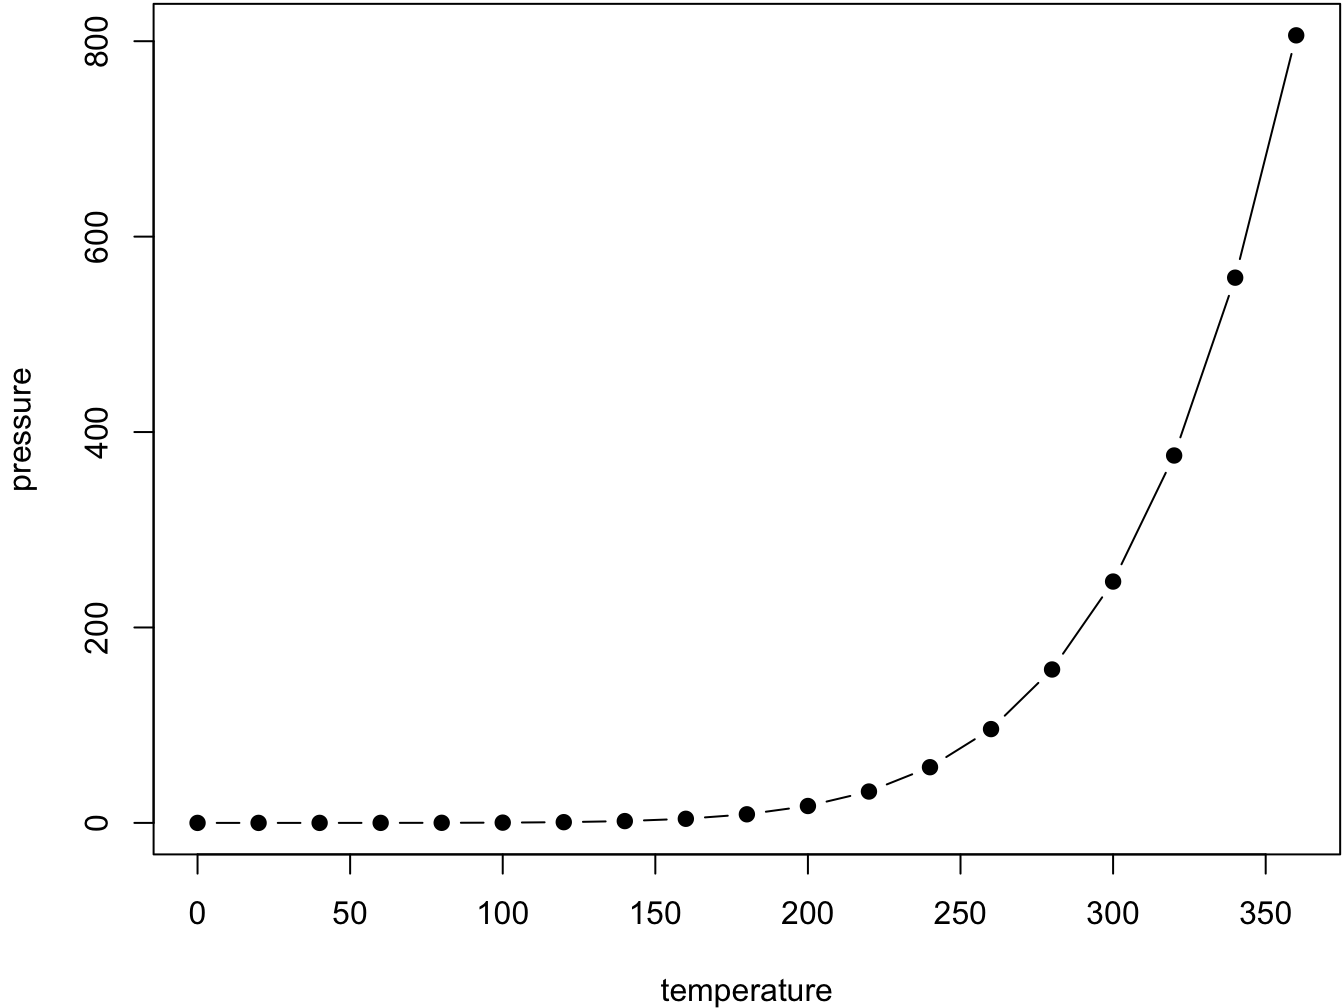
\includegraphics{figures/fig.png}
\caption{image}
\end{figure}

En modifiant la largeur: 200px

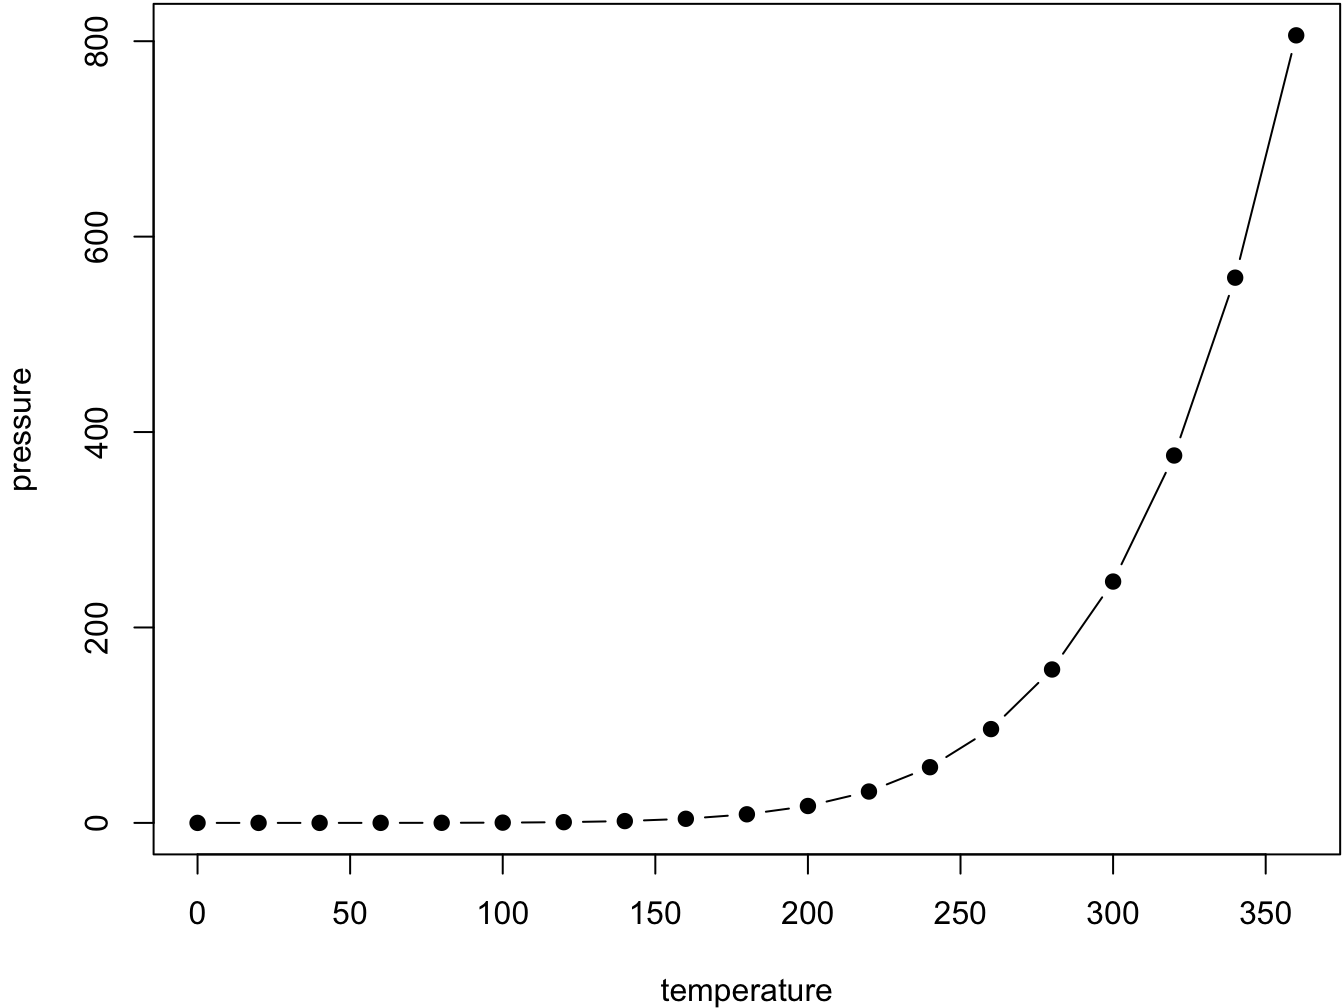
\includegraphics{figures/fig.png}\{width: 200px;\}

En utilisant knitr:

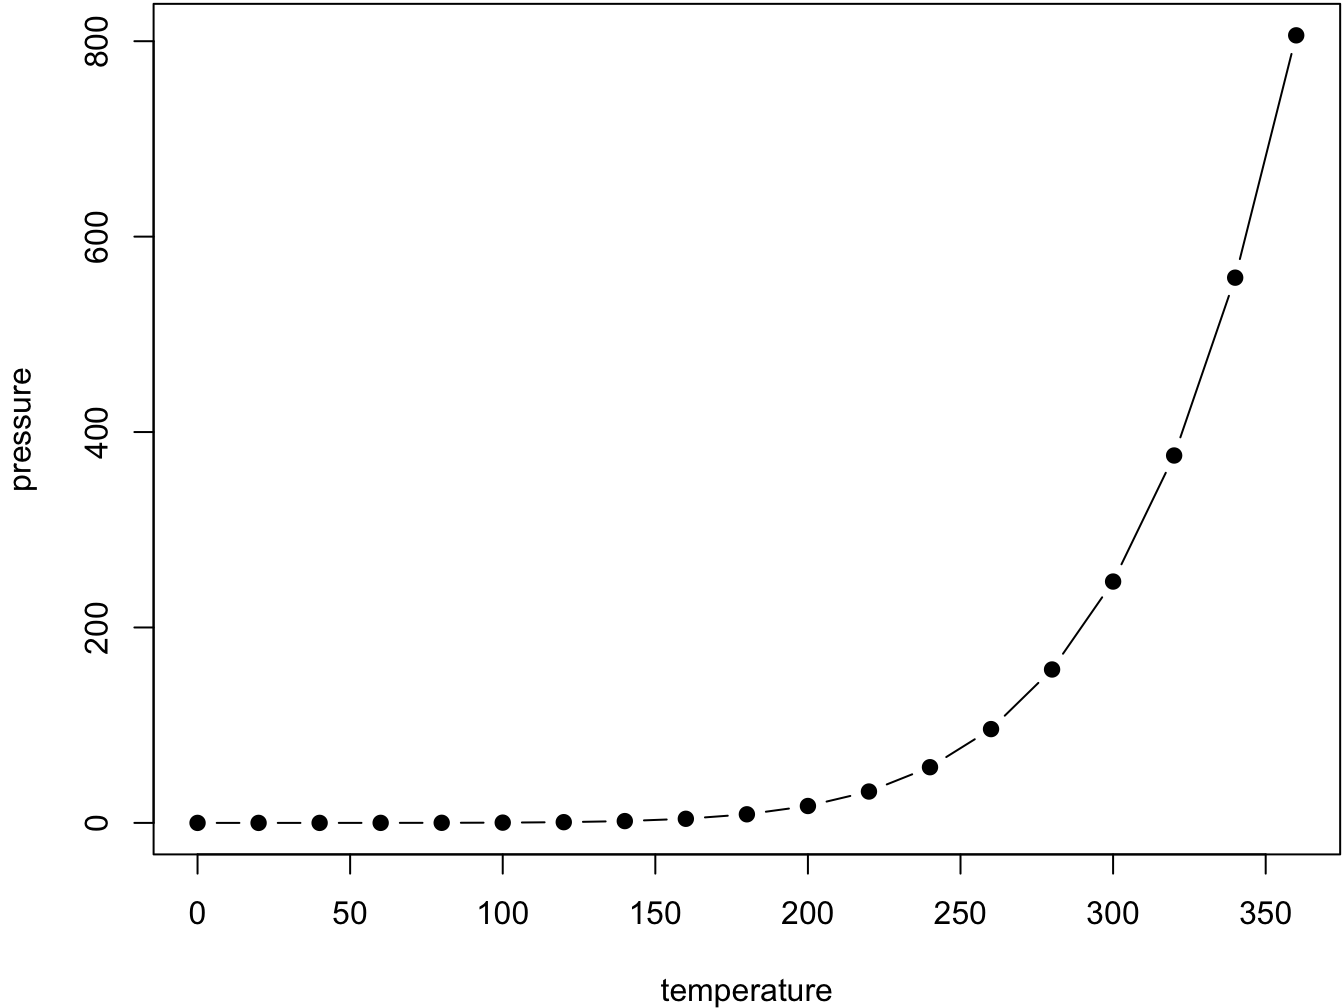
\includegraphics[width=0.5\linewidth]{figures/fig}

Figures and tables with captions will be placed in \texttt{figure} and \texttt{table} environments, respectively

\begin{Shaded}
\begin{Highlighting}[]
\NormalTok{knitr}\SpecialCharTok{::}\FunctionTok{include\_graphics}\NormalTok{(}\StringTok{"figures/fig.png"}\NormalTok{)}
\end{Highlighting}
\end{Shaded}

\begin{figure}

{\centering 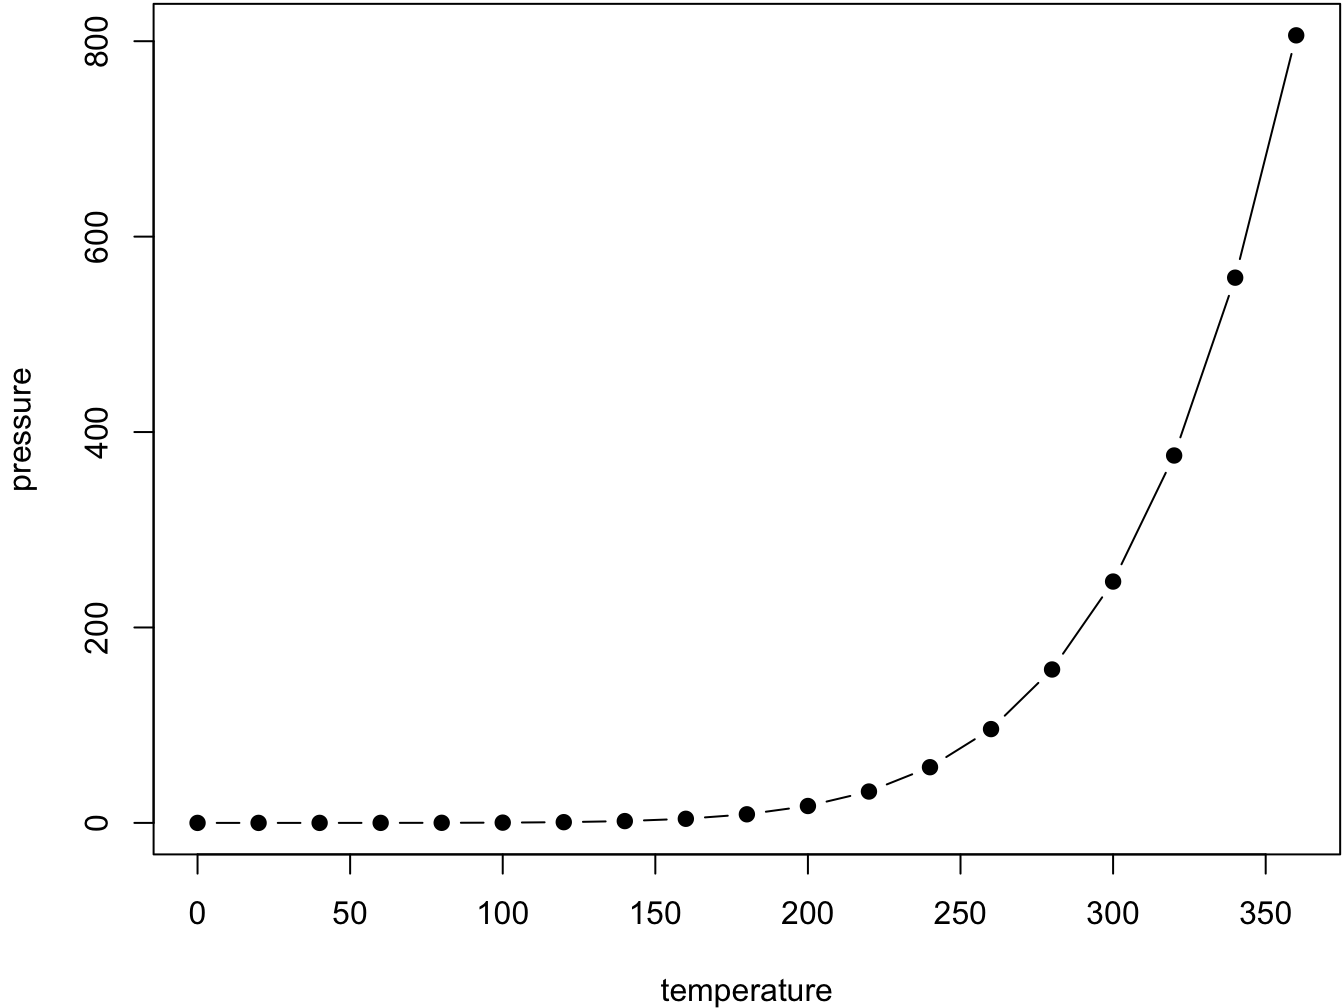
\includegraphics[width=0.6\linewidth]{figures/fig} 

}

\caption{Here is a nice figure!}\label{fig:nice-fig}
\end{figure}

\newpage

Figures and tables with captions will be placed in \texttt{figure} and \texttt{table} environments, respectively

\begin{Shaded}
\begin{Highlighting}[]
\NormalTok{knitr}\SpecialCharTok{::}\FunctionTok{include\_graphics}\NormalTok{(}\StringTok{"figures/fig.png"}\NormalTok{)}
\end{Highlighting}
\end{Shaded}

\begin{figure}

{\centering 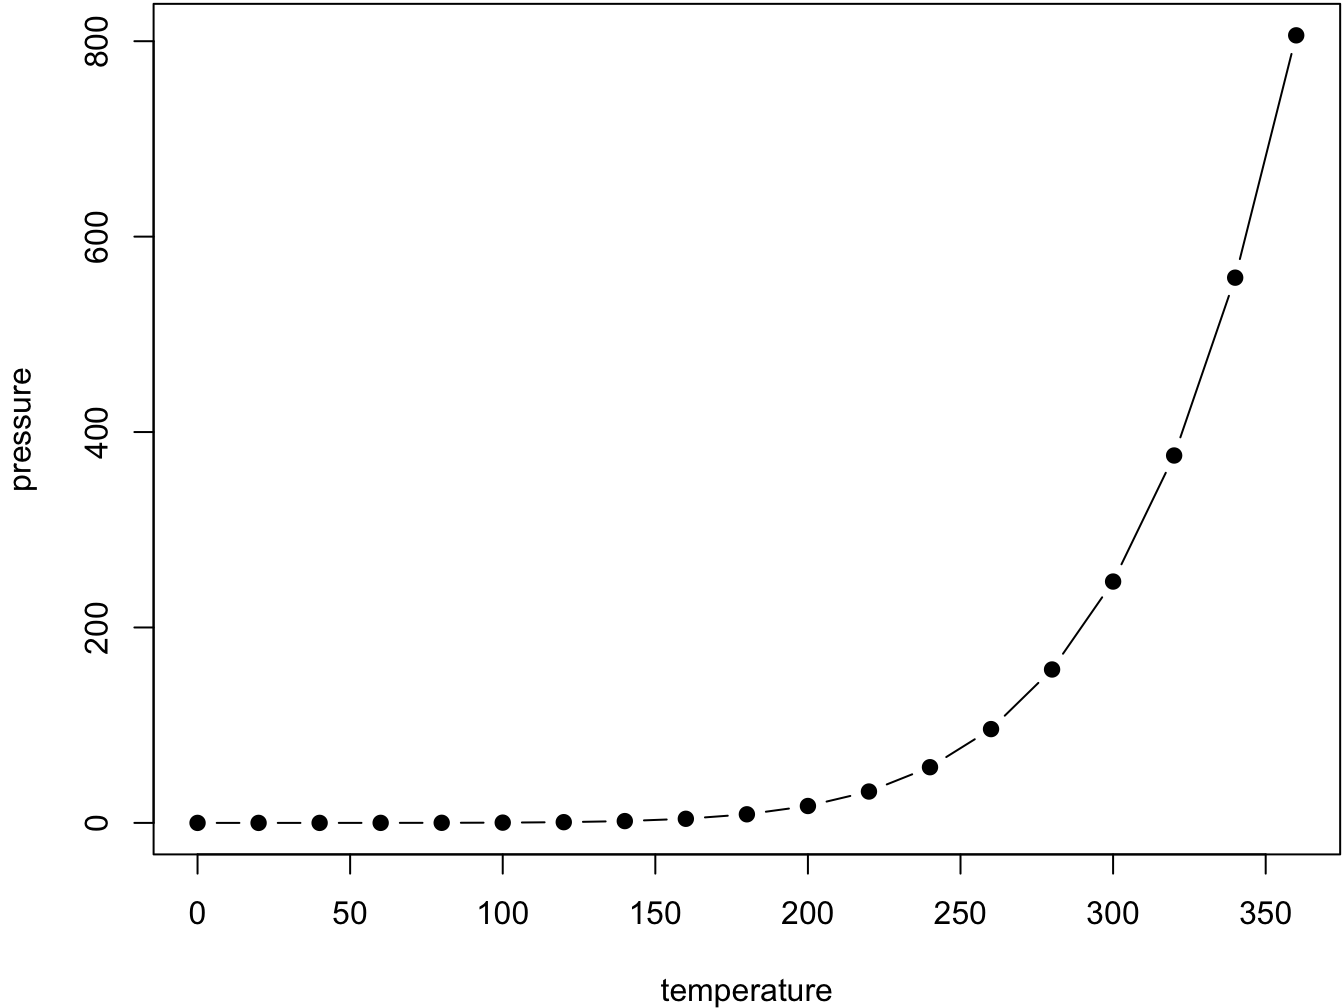
\includegraphics[width=0.8\linewidth]{figures/fig} 

}

\caption{Here is a nice figure!}\label{fig:unnamed-chunk-9}
\end{figure}

\hypertarget{rappel-de-chimie}{%
\chapter{Rappel de chimie}\label{rappel-de-chimie}}

Liste des notions:

\begin{itemize}
\tightlist
\item
  Dissolution (composé moléculaire / ionique)
\item
  Solution
\item
  Concentration
\item
  Dilution
\item
  Fiche ions, molécules à connaître
\end{itemize}

\hypertarget{literature}{%
\chapter{Literature}\label{literature}}

Here is a review of existing methods.

\hypertarget{methods}{%
\chapter{Methods}\label{methods}}

We describe our methods in this chapter.

\hypertarget{applications}{%
\chapter{Applications}\label{applications}}

Some \emph{significant} applications are demonstrated in this chapter.

\hypertarget{example-one}{%
\section{Example one}\label{example-one}}

\hypertarget{example-two}{%
\section{Example two}\label{example-two}}

\hypertarget{final-words}{%
\chapter{Final Words}\label{final-words}}

We have finished a nice book.

  \bibliography{book.bib,packages.bib}

\end{document}
